\batchmode

\documentclass[11pt,a4paper]{article}
\RequirePackage{ifthen}


\usepackage{epsfig}
\usepackage[utf8]{inputenc}
\usepackage[english]{babel}
\usepackage{listings}
\usepackage{html}


\lstset{%basicstyle=\scriptsize\ttfamily,
	basicstyle=\small ,
        tabsize=2,
	float=tbph,
        showspaces=false,
	aboveskip=\bigskipamount,
        numbers=left,
        numberstyle=\tiny , 
	breaklines=true,
        stepnumber=2, 
        numbersep=5pt,
        captionpos=b}



\setlength{\topmargin}{-13mm} 

\setlength{\oddsidemargin}{5mm} 

\setlength{\evensidemargin}{5mm} 

\setlength{\textwidth}{155mm}  

\setlength{\textheight}{230mm} 



\setlength{\abovecaptionskip}{-2pt} 




\usepackage[dvips]{color}


\pagecolor[gray]{.7}

\usepackage[]{inputenc}



\makeatletter

\makeatletter
\count@=\the\catcode`\_ \catcode`\_=8 
\newenvironment{tex2html_wrap}{}{}%
\catcode`\<=12\catcode`\_=\count@
\newcommand{\providedcommand}[1]{\expandafter\providecommand\csname #1\endcsname}%
\newcommand{\renewedcommand}[1]{\expandafter\providecommand\csname #1\endcsname{}%
  \expandafter\renewcommand\csname #1\endcsname}%
\newcommand{\newedenvironment}[1]{\newenvironment{#1}{}{}\renewenvironment{#1}}%
\let\newedcommand\renewedcommand
\let\renewedenvironment\newedenvironment
\makeatother
\let\mathon=$
\let\mathoff=$
\ifx\AtBeginDocument\undefined \newcommand{\AtBeginDocument}[1]{}\fi
\newbox\sizebox
\setlength{\hoffset}{0pt}\setlength{\voffset}{0pt}
\addtolength{\textheight}{\footskip}\setlength{\footskip}{0pt}
\addtolength{\textheight}{\topmargin}\setlength{\topmargin}{0pt}
\addtolength{\textheight}{\headheight}\setlength{\headheight}{0pt}
\addtolength{\textheight}{\headsep}\setlength{\headsep}{0pt}
\setlength{\textwidth}{349pt}
\newwrite\lthtmlwrite
\makeatletter
\let\realnormalsize=\normalsize
\global\topskip=2sp
\def\preveqno{}\let\real@float=\@float \let\realend@float=\end@float
\def\@float{\let\@savefreelist\@freelist\real@float}
\def\liih@math{\ifmmode$\else\bad@math\fi}
\def\end@float{\realend@float\global\let\@freelist\@savefreelist}
\let\real@dbflt=\@dbflt \let\end@dblfloat=\end@float
\let\@largefloatcheck=\relax
\let\if@boxedmulticols=\iftrue
\def\@dbflt{\let\@savefreelist\@freelist\real@dbflt}
\def\adjustnormalsize{\def\normalsize{\mathsurround=0pt \realnormalsize
 \parindent=0pt\abovedisplayskip=0pt\belowdisplayskip=0pt}%
 \def\phantompar{\csname par\endcsname}\normalsize}%
\def\lthtmltypeout#1{{\let\protect\string \immediate\write\lthtmlwrite{#1}}}%
\newcommand\lthtmlhboxmathA{\adjustnormalsize\setbox\sizebox=\hbox\bgroup\kern.05em }%
\newcommand\lthtmlhboxmathB{\adjustnormalsize\setbox\sizebox=\hbox to\hsize\bgroup\hfill }%
\newcommand\lthtmlvboxmathA{\adjustnormalsize\setbox\sizebox=\vbox\bgroup %
 \let\ifinner=\iffalse \let\)\liih@math }%
\newcommand\lthtmlboxmathZ{\@next\next\@currlist{}{\def\next{\voidb@x}}%
 \expandafter\box\next\egroup}%
\newcommand\lthtmlmathtype[1]{\gdef\lthtmlmathenv{#1}}%
\newcommand\lthtmllogmath{\lthtmltypeout{l2hSize %
:\lthtmlmathenv:\the\ht\sizebox::\the\dp\sizebox::\the\wd\sizebox.\preveqno}}%
\newcommand\lthtmlfigureA[1]{\let\@savefreelist\@freelist
       \lthtmlmathtype{#1}\lthtmlvboxmathA}%
\newcommand\lthtmlpictureA{\bgroup\catcode`\_=8 \lthtmlpictureB}%
\newcommand\lthtmlpictureB[1]{\lthtmlmathtype{#1}\egroup
       \let\@savefreelist\@freelist \lthtmlhboxmathB}%
\newcommand\lthtmlpictureZ[1]{\hfill\lthtmlfigureZ}%
\newcommand\lthtmlfigureZ{\lthtmlboxmathZ\lthtmllogmath\copy\sizebox
       \global\let\@freelist\@savefreelist}%
\newcommand\lthtmldisplayA{\bgroup\catcode`\_=8 \lthtmldisplayAi}%
\newcommand\lthtmldisplayAi[1]{\lthtmlmathtype{#1}\egroup\lthtmlvboxmathA}%
\newcommand\lthtmldisplayB[1]{\edef\preveqno{(\theequation)}%
  \lthtmldisplayA{#1}\let\@eqnnum\relax}%
\newcommand\lthtmldisplayZ{\lthtmlboxmathZ\lthtmllogmath\lthtmlsetmath}%
\newcommand\lthtmlinlinemathA{\bgroup\catcode`\_=8 \lthtmlinlinemathB}
\newcommand\lthtmlinlinemathB[1]{\lthtmlmathtype{#1}\egroup\lthtmlhboxmathA
  \vrule height1.5ex width0pt }%
\newcommand\lthtmlinlineA{\bgroup\catcode`\_=8 \lthtmlinlineB}%
\newcommand\lthtmlinlineB[1]{\lthtmlmathtype{#1}\egroup\lthtmlhboxmathA}%
\newcommand\lthtmlinlineZ{\egroup\expandafter\ifdim\dp\sizebox>0pt %
  \expandafter\centerinlinemath\fi\lthtmllogmath\lthtmlsetinline}
\newcommand\lthtmlinlinemathZ{\egroup\expandafter\ifdim\dp\sizebox>0pt %
  \expandafter\centerinlinemath\fi\lthtmllogmath\lthtmlsetmath}
\newcommand\lthtmlindisplaymathZ{\egroup %
  \centerinlinemath\lthtmllogmath\lthtmlsetmath}
\def\lthtmlsetinline{\hbox{\vrule width.1em \vtop{\vbox{%
  \kern.1em\copy\sizebox}\ifdim\dp\sizebox>0pt\kern.1em\else\kern.3pt\fi
  \ifdim\hsize>\wd\sizebox \hrule depth1pt\fi}}}
\def\lthtmlsetmath{\hbox{\vrule width.1em\kern-.05em\vtop{\vbox{%
  \kern.1em\kern0.8 pt\hbox{\hglue.17em\copy\sizebox\hglue0.8 pt}}\kern.3pt%
  \ifdim\dp\sizebox>0pt\kern.1em\fi \kern0.8 pt%
  \ifdim\hsize>\wd\sizebox \hrule depth1pt\fi}}}
\def\centerinlinemath{%
  \dimen1=\ifdim\ht\sizebox<\dp\sizebox \dp\sizebox\else\ht\sizebox\fi
  \advance\dimen1by.5pt \vrule width0pt height\dimen1 depth\dimen1 
 \dp\sizebox=\dimen1\ht\sizebox=\dimen1\relax}

\def\lthtmlcheckvsize{\ifdim\ht\sizebox<\vsize 
  \ifdim\wd\sizebox<\hsize\expandafter\hfill\fi \expandafter\vfill
  \else\expandafter\vss\fi}%
\providecommand{\selectlanguage}[1]{}%
\makeatletter \tracingstats = 1 


\begin{document}
\pagestyle{empty}\thispagestyle{empty}\lthtmltypeout{}%
\lthtmltypeout{latex2htmlLength hsize=\the\hsize}\lthtmltypeout{}%
\lthtmltypeout{latex2htmlLength vsize=\the\vsize}\lthtmltypeout{}%
\lthtmltypeout{latex2htmlLength hoffset=\the\hoffset}\lthtmltypeout{}%
\lthtmltypeout{latex2htmlLength voffset=\the\voffset}\lthtmltypeout{}%
\lthtmltypeout{latex2htmlLength topmargin=\the\topmargin}\lthtmltypeout{}%
\lthtmltypeout{latex2htmlLength topskip=\the\topskip}\lthtmltypeout{}%
\lthtmltypeout{latex2htmlLength headheight=\the\headheight}\lthtmltypeout{}%
\lthtmltypeout{latex2htmlLength headsep=\the\headsep}\lthtmltypeout{}%
\lthtmltypeout{latex2htmlLength parskip=\the\parskip}\lthtmltypeout{}%
\lthtmltypeout{latex2htmlLength oddsidemargin=\the\oddsidemargin}\lthtmltypeout{}%
\makeatletter
\if@twoside\lthtmltypeout{latex2htmlLength evensidemargin=\the\evensidemargin}%
\else\lthtmltypeout{latex2htmlLength evensidemargin=\the\oddsidemargin}\fi%
\lthtmltypeout{}%
\makeatother
\setcounter{page}{1}
\onecolumn

% !!! IMAGES START HERE !!!

\stepcounter{section}
{\newpage\clearpage
\lthtmlfigureA{figure87}%
\begin{figure}\centering
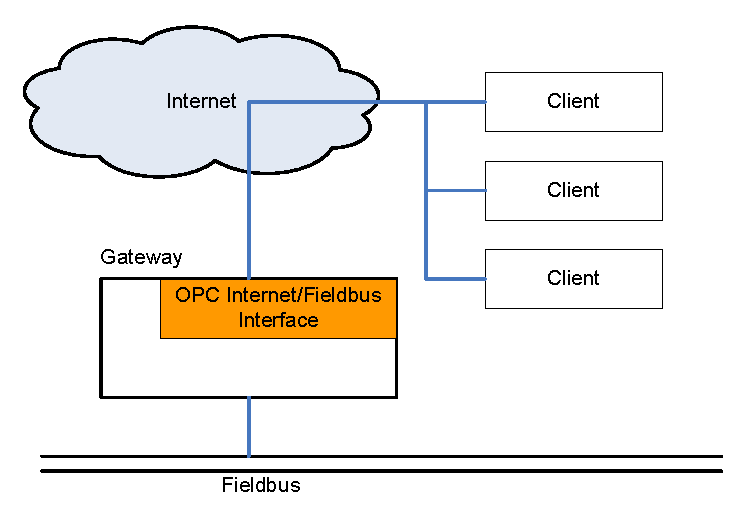
\includegraphics[scale=0.7]{graphics/inet_fb_gw.eps}

\end{figure}%
\lthtmlfigureZ
\lthtmlcheckvsize\clearpage}

\stepcounter{section}
{\newpage\clearpage
\lthtmlfigureA{lstlisting155}%
\begin{lstlisting}[caption={Accessing a remote OPC XML-DA server}
                   ,label=ex_quickstart] 
from PyOPC.XDAClient import XDAClient
\par
address='http://path/to/server'
xda = XDAClient(OPCServerAddress=address)
xda.GetStatus()
\end{lstlisting}%
\lthtmlfigureZ
\lthtmlcheckvsize\clearpage}

\stepcounter{section}
{\newpage\clearpage
\lthtmlfigureA{figure196}%
\begin{figure}\centering
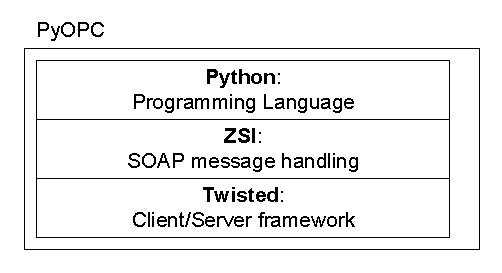
\includegraphics[scale=0.7]{graphics/technologies.eps}

\end{figure}%
\lthtmlfigureZ
\lthtmlcheckvsize\clearpage}

\stepcounter{subsection}
{\newpage\clearpage
\lthtmlfigureA{figure211}%
\begin{figure}\centering
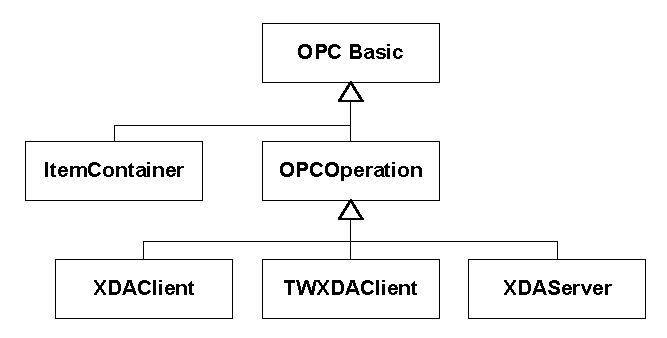
\includegraphics[scale=0.7]{graphics/object_hierarchy.eps}

\end{figure}%
\lthtmlfigureZ
\lthtmlcheckvsize\clearpage}

\stepcounter{subsection}
{\newpage\clearpage
\lthtmlfigureA{figure222}%
\begin{figure}\centering
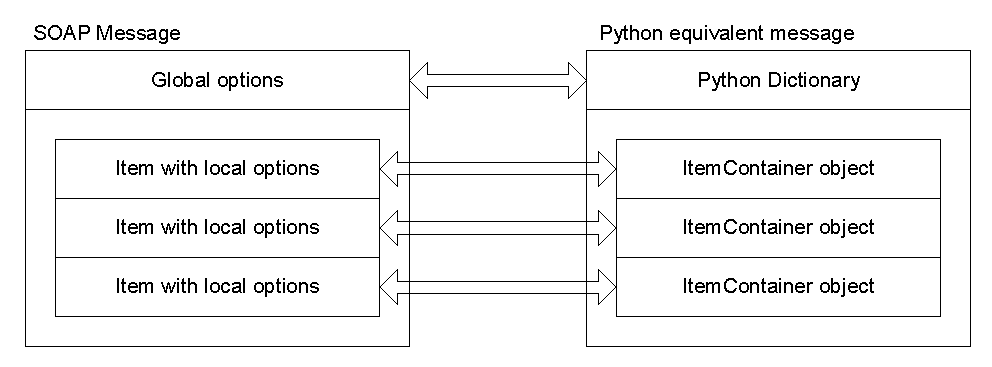
\includegraphics[scale=0.7]{graphics/message_basic.eps}

\end{figure}%
\lthtmlfigureZ
\lthtmlcheckvsize\clearpage}

{\newpage\clearpage
\lthtmlfigureA{lstlisting230}%
\begin{lstlisting}[caption={Usage of Python objects for representing
global and local options of a OPC XML-DA compliant SOAP message}
                   ,label=ex_message_basic] 
item = ItemContainer(ItemName='test_name', MaxAge=500)
item_list,global_options = xda.Read([item], ItemPath='test_path')
\end{lstlisting}%
\lthtmlfigureZ
\lthtmlcheckvsize\clearpage}

{\newpage\clearpage
\lthtmlfigureA{lstlisting237}%
\begin{lstlisting}[caption={Assigning Global Options to a PyOPC 
Client Instance}
                   ,label=ex_global]
xda = XDAClient(ReturnErrorText=False,
                ReturnItemName=True,
                ReturnDiagnosticInfo=True,
                ItemPath='')
\end{lstlisting}%
\lthtmlfigureZ
\lthtmlcheckvsize\clearpage}

{\newpage\clearpage
\lthtmlfigureA{lstlisting244}%
\begin{lstlisting}[caption={Accessing the PyOPC ItemContainer Object}
                   ,label=ex_itemcontainer] 
from PyOPC.OPCContainers import *
item = ItemContainer(ItemName='test_name',
                     MaxAge=500)
item.ItemName='other_name'
maxage = item.MaxAge
\end{lstlisting}%
\lthtmlfigureZ
\lthtmlcheckvsize\clearpage}

{\newpage\clearpage
\lthtmlfigureA{lstlisting260}%
\begin{lstlisting}[caption={Handling Qualified Names (QNames) with PyOPC}
                   ,label=ex_qnames] 
from PyOPC.utils import *
\par
qn1 = QName(NS\_XSD,'string')
qn2 = QName('http://my/name/space','test123')
url, name = qn2.URI, qn2.name
\end{lstlisting}%
\lthtmlfigureZ
\lthtmlcheckvsize\clearpage}

{\newpage\clearpage
\lthtmlfigureA{lstlisting273}%
\begin{lstlisting}[caption={Creating and Accessing PyOPC Properties}
                   ,label=ex_properties] 
p1 = OPCProperty(Name = QName(NS_XDA,'accessRights'),
                 Value = 'readable',
                 Description = 'Access Rights')
print p1.Name, p1.Value
p1.ItemPath = 'MyPath'                 
\par
p2 = OPCProperty(Name = 'accessRights')
print p2.Description
\end{lstlisting}%
\lthtmlfigureZ
\lthtmlcheckvsize\clearpage}

{\newpage\clearpage
\lthtmlfigureA{table288}%
\begin{table}\centering
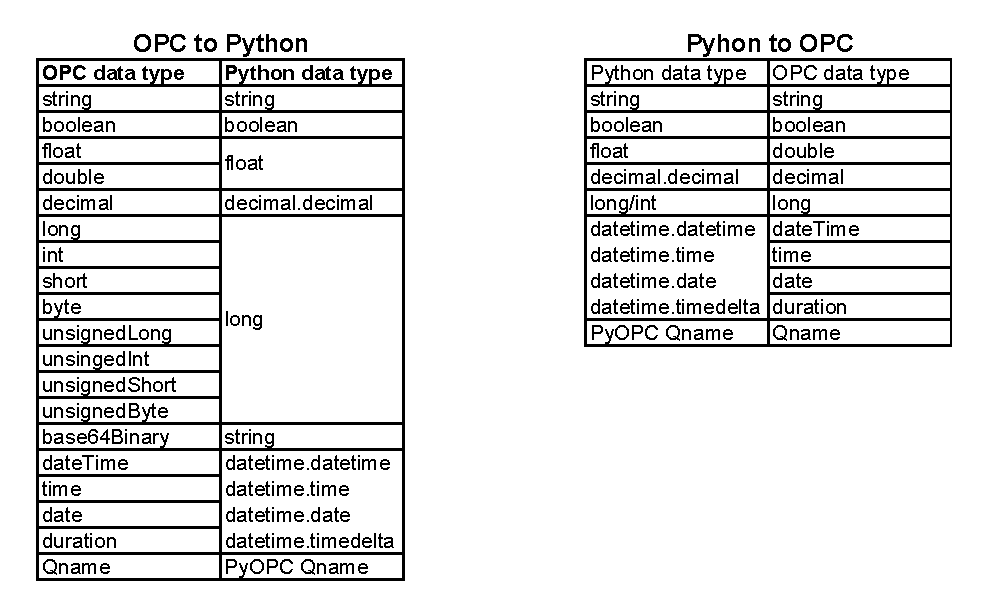
\includegraphics[scale=0.7]{graphics/dataconv.eps}

\end{table}%
\lthtmlfigureZ
\lthtmlcheckvsize\clearpage}

\stepcounter{subsection}
\stepcounter{section}
\stepcounter{subsection}
{\newpage\clearpage
\lthtmlfigureA{lstlisting565}%
\begin{lstlisting}[caption={Sample client code based on the PyOPC XDAClient 
module}
                   ,label=ex_xdaclient] 
from PyOPC.OPCContainers import *
from PyOPC.XDAClient import XDAClient
\par
def print_options((ilist,options)):
    print ilist; print options; print
\par
address='http://violin.qwer.tk:8000/'
\par
xda = XDAClient(OPCServerAddress=address,
                ReturnErrorText=True)
\par
print_options(xda.GetStatus())
print_options(xda.Browse())
print_options(xda.Read([ItemContainer(ItemName='simple_item', 
                                      MaxAge=500)], 
                       LocaleID='en-us'))
\end{lstlisting}%
\lthtmlfigureZ
\lthtmlcheckvsize\clearpage}

\stepcounter{subsection}
{\newpage\clearpage
\lthtmlfigureA{lstlisting580}%
\begin{lstlisting}[caption={Sample client code based on the PyOPC TWXDAClient 
module}
                   ,label=ex_twxdaclient] 
from PyOPC.OPCContainers import *
from PyOPC.TWXDAClient import TWXDAClient
from twisted.internet import reactor
\par
OPERATIONS = 3
\par
def print_options((ilist,options)):
    print ilist; print options; print
    global OPERATIONS
    OPERATIONS -= 1
    if OPERATIONS == 0:
        reactor.stop()
\par
def handleError(failure):
    print "An Error occured"
    print failure.getTraceback()
    reactor.stop()
\par
address='http://violin.qwer.tk:8000/'
\par
xda = TWXDAClient(OPCServerAddress=address,
                ReturnErrorText=True)
\par
d = xda.twGetStatus()
d.addCallback(print_options)
d.addErrback(handleError)
\par
d = xda.twBrowse()
d.addCallback(print_options)
d.addErrback(handleError)
\par
d = xda.twRead([ItemContainer(ItemName='simple_item', MaxAge=500)],
               LocaleID='en-us')
d.addCallback(print_options)
d.addErrback(handleError)
\par
reactor.run()
\end{lstlisting}%
\lthtmlfigureZ
\lthtmlcheckvsize\clearpage}

\stepcounter{section}
{\newpage\clearpage
\lthtmlfigureA{figure696}%
\begin{figure}\centering
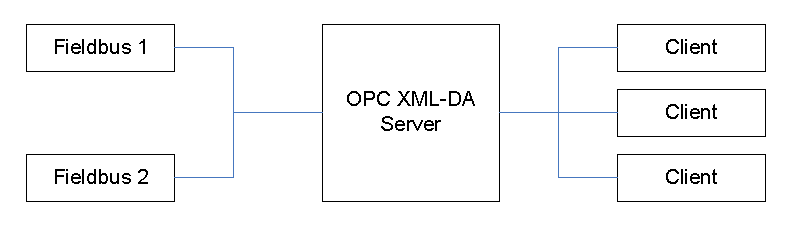
\includegraphics[scale=0.7]{graphics/opc_proxy.eps}

\end{figure}%
\lthtmlfigureZ
\lthtmlcheckvsize\clearpage}

{\newpage\clearpage
\lthtmlfigureA{figure704}%
\begin{figure}\centering
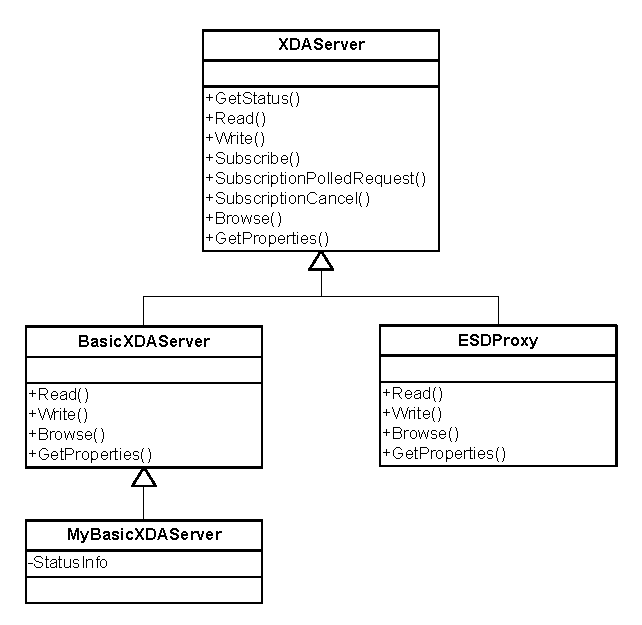
\includegraphics[scale=0.7]{graphics/server_hierarchy.eps}

\end{figure}%
\lthtmlfigureZ
\lthtmlcheckvsize\clearpage}

{\newpage\clearpage
\lthtmlfigureA{lstlisting717}%
\begin{lstlisting}[caption={Simple OPC XML-DA Server}
                   ,label=ex_simple_server] 
import random
from twisted.internet import reactor,defer
from PyOPC.servers.basic import BasicXDAServer
\par
# Read sample OPC items for testing
import sample_items
\par
class MyXDAServer(BasicXDAServer):
    OPCItems = sample_items.TestOPCItems
    StatusInfo = 'My Basic OPC XML-DA Server'
\par
def GetStatus(self, (IPH,inOptions,outOptions)):
        ''' Custom GetStatus that alters the Product Version'''
\par
outOptions['ProductVersion'] = str(random.choice(range(1,10)))
\par
return super(MyXDAServer, self).GetStatus((IPH,inOptions,outOptions))
\end{lstlisting}%
\lthtmlfigureZ
\lthtmlcheckvsize\clearpage}

{\newpage\clearpage
\lthtmlfigureA{figure721}%
\begin{figure}\centering
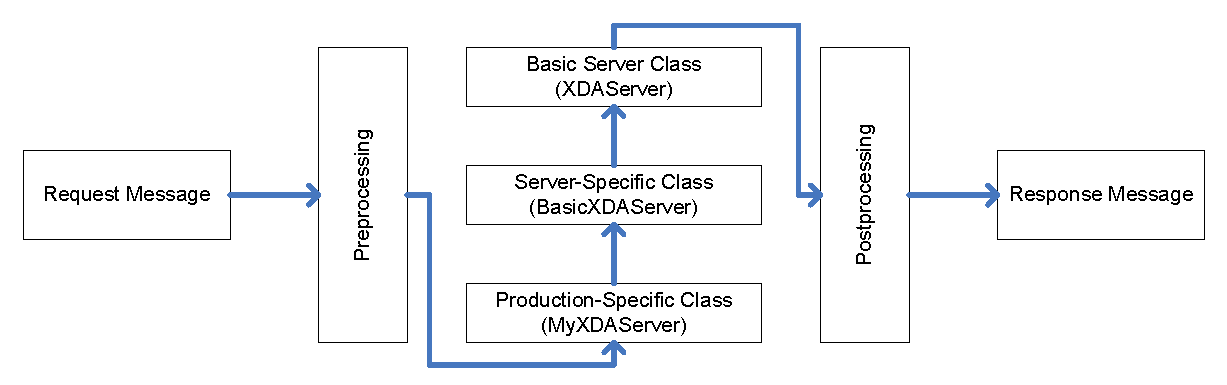
\includegraphics[scale=0.7]{graphics/opc_parameters.eps}

\end{figure}%
\lthtmlfigureZ
\lthtmlcheckvsize\clearpage}

{\newpage\clearpage
\lthtmlfigureA{lstlisting732}%
\begin{lstlisting}[caption={Creating and Managing the ItemPairHolder object}
                   ,label=ex_IPH] 
IPH = ItemPairHolder()
IPH.append(inItem, outItem)
for inItem, outItem in IPH:
   outItem.ItemPath = inItem.ItemPath
\end{lstlisting}%
\lthtmlfigureZ
\lthtmlcheckvsize\clearpage}

\stepcounter{subsection}
\stepcounter{subsection}
{\newpage\clearpage
\lthtmlfigureA{figure766}%
\begin{figure}\centering
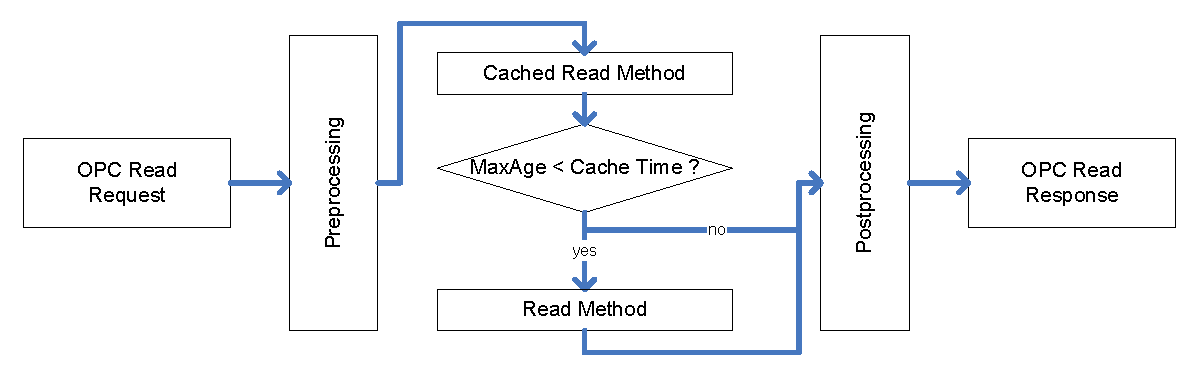
\includegraphics[scale=0.7]{graphics/item_caching.eps}

\end{figure}%
\lthtmlfigureZ
\lthtmlcheckvsize\clearpage}

{\newpage\clearpage
\lthtmlfigureA{figure777}%
\begin{figure}\centering
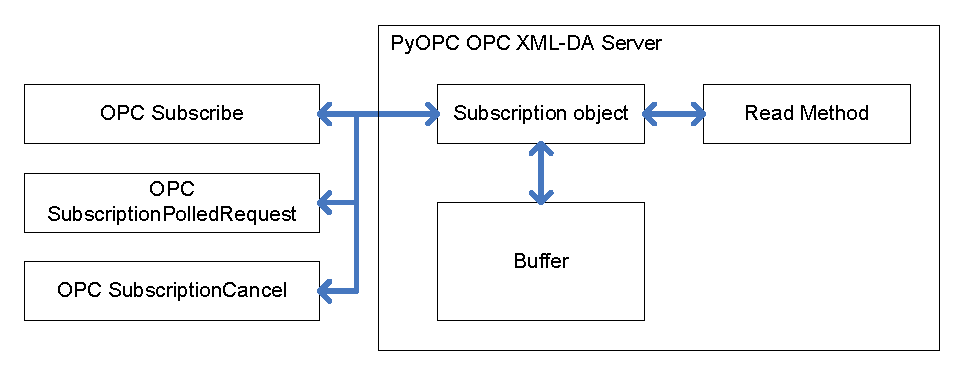
\includegraphics[scale=0.7]{graphics/pyopc_subs.eps}

\end{figure}%
\lthtmlfigureZ
\lthtmlcheckvsize\clearpage}

\stepcounter{subsection}
{\newpage\clearpage
\lthtmlfigureA{lstlisting811}%
\begin{lstlisting}[caption={Instantiating and Starting a PyOPC-based
OPC XML-DA Server}
                   ,label=ex_start] 
from twisted.web import resource, server
xdasrv = MyXDAServer(http_log_fn = 'http.log')
root = resource.Resource()
root.putChild('',xdasrv)
site = server.Site(root)
reactor.listenTCP(8000, site)
reactor.run()
\end{lstlisting}%
\lthtmlfigureZ
\lthtmlcheckvsize\clearpage}

{\newpage\clearpage
\lthtmlfigureA{lstlisting816}%
\begin{lstlisting}[caption={Adding Multiple PyOPC Server Objects to
One Twisted Resource}
                   ,label=ex_multiserver] 
root = resource.Resource()
root.putChild('srv1',MyXDAServer1())
root.putChild('srv2',MyXDAServer2())
root.putChild('srv3',MyXDAServer3())
\end{lstlisting}%
\lthtmlfigureZ
\lthtmlcheckvsize\clearpage}

\stepcounter{subsection}
{\newpage\clearpage
\lthtmlfigureA{lstlisting823}%
\begin{lstlisting}[caption={PyOPC server based on the class 
BasicXDAServer}
                   ,label=ex_basicxdaserver] 
class MyXDAServer(BasicXDAServer):
    OPCItems = (ItemContainer(ItemName='sample_integer',
                               Value=14,
                               QualityField='good'),
                ItemContainer(ItemName='sample_float',
                               Value=96.43,
                               QualityField='good'))
\end{lstlisting}%
\lthtmlfigureZ
\lthtmlcheckvsize\clearpage}

\stepcounter{section}
{\newpage\clearpage
\lthtmlfigureA{table1128}%
\begin{table}\centering
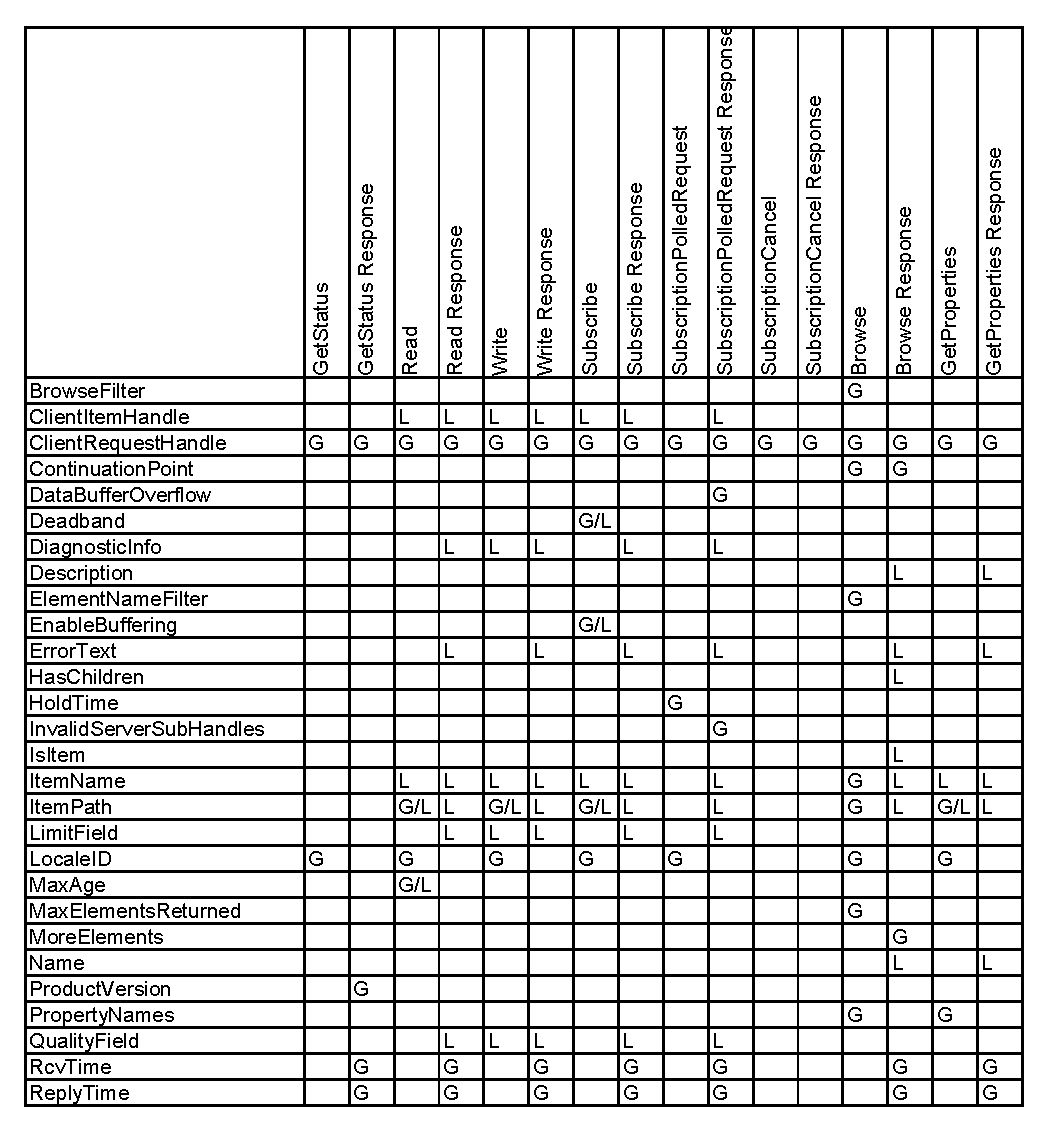
\includegraphics[scale=0.9]{graphics/operations1.eps}

\end{table}%
\lthtmlfigureZ
\lthtmlcheckvsize\clearpage}

{\newpage\clearpage
\lthtmlfigureA{table1134}%
\begin{table}\centering
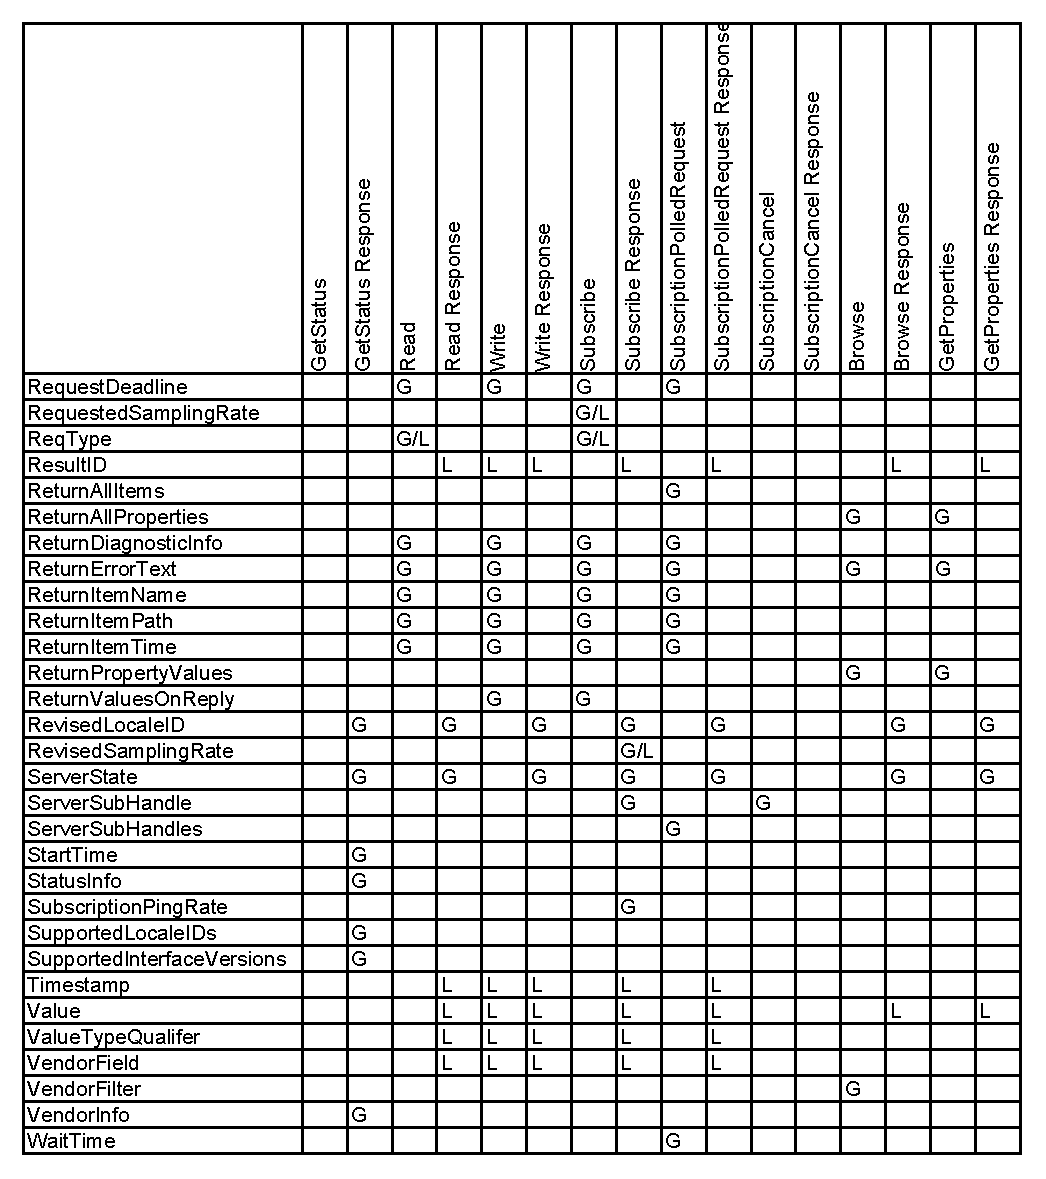
\includegraphics[scale=0.9]{graphics/operations2.eps}

\end{table}%
\lthtmlfigureZ
\lthtmlcheckvsize\clearpage}


\end{document}
